\documentclass[minted]{protocol}
% Required
\title{Komplexe komponentenbasierte Programmierung}
\author{Ebenstein Michael}
% Optional
\mysubtitle{Laborprotokoll}
\mysubject{Systemtechnik Labor}
\mycourse{4BHIT 2017/18, Gruppe B}
% Version
\myteacher{Michael Borko}
\myversion{1.1}
\mybegin{10. Juni 2018}
\myfinish{13. Juni 2018}
% \setcode{frame=single} 			% Add a frame to codes (single, lines)
% \setcode{bgcolor=MyLightGray}		% Add a background to codes (minted only)
% \usemintedstyle{rainbow_dash} 	% autumn, rainbow_dash, tango (default), trac
\begin{document}
% \thispagestyle{fancy}				% Makes the first page fancy too
% \begin{abstract}\end{abstract} 	% Add a short overview
\section{Einführung}
Diese Übung zeigt die Anwendung von komponentenbasierter Programmierung mittels Webframeworks.
\subsection{Ziele}

Das Ziel dieser Übung ist die Umsetzung einer View sowie die Implementierung von Business-Logic mittels eines Frameworks.
\subsection{Voraussetzungen} 

Grundlagen zu Java und das Anwenden neuer Application Programming Interfaces (APIs)
Abgeschlossene Implementierung der Übung Distributed Computing DezSys-GK8.3 "Komponentenbasierte Programmierung"
\subsection{Aufgabenstellung}

Erstellen Sie für die persistierten Objekte des Modells eine grafische Oberfläche mit einem Webframework. Die funktionalen Anforderungen, die infolge beschrieben sind, sollen entsprechend abgebildet sein.

\subsubsection{Suche}
Die Suche nach Zügen muss auf jeden Fall die Auswahl des Abfahrts- und Ankunftsortes (nur folgende Bahnhöfe sind möglich: Wien Westbhf, Wien Hütteldorf, St. Pölten, Amstetten, Linz, Wels, Attnang-Puchheim, Salzburg) ermöglichen. Dies führt zur Anzeige der möglichen Abfahrten, die zur Vereinfachung an jedem Tag zur selben Zeit stattfinden. Des weiteren wird auch die Dauer der Fahrt angezeigt.

In dieser Liste kann nun eine gewünschte Abfahrtszeit ausgewählt werden. Die Auswahl der Zeit führt zu einer automatischen Weiterleitung zum Ticketshop.

Um sich die Auslastung der reservierten Sitzplätze anzusehen, muss bei dem Suchlisting noch das Datum ausgewählt werden. Dieses Service steht jedoch nur registrierten Benutzern zur Verfügung.


\subsubsection{Ticketshop}
Man kann Einzeltickets kaufen, Reservierungen für bestimmte Züge durchführen und Zeitkarten erwerben. Dabei sind folgende Angaben notwendig:

Einzeltickets: Strecke (Abfahrt/Ankunft), Anzahl der Tickets, Optionen (Fahrrad, Großgepäck)
Reservierung: Strecke (Abfahrt/Ankunft), Art der Reservierung (Sitzplatz, Fahrrad, Rollstuhlstellplatz), Reisetag und Zug (Datum/Uhrzeit)
Zeitkarte: Strecke, Zeitraum (Wochen- und Monatskarte)

Um einen Überblick zu erhalten, kann der Warenkorb beliebig befüllt und jederzeit angezeigt werden. Es sind keine Änderungen erlaubt, jedoch können einzelne Posten wieder gelöscht werden.

Die Funktion „Zur Kassa gehen“ soll die Bezahlung und den Ausdruck der Tickets sowie die Zusendung per eMail/SMS ermöglichen. Dabei ist für die Bezahlung nur ein Schein-Service zu verwenden um zum Beispiel eine Kreditkarten- bzw. Maestrotransaktion zu simulieren.

\subsubsection{Prämienmeilen}

Benutzer können sich am System registrieren um getätigte Käufe und Reservierungen einzusehen. Diese führen nämlich zu Prämienmeilen, die weitere Vergünstigungen ermöglichen. Um diese beim nächsten Einkauf nützen zu können, muss sich der Benutzer einloggen und wird beim „Zur Kassa gehen“ gefragt, ob er die Prämienmeilen für diesen Kauf einlösen möchte.

Instant Notification System der Warteliste
Der Kunde soll über Änderungen bezüglich seiner Reservierung (Verspätung bzw. Stornierung) mittels ausgesuchtem Service (eMail bzw. SMS) benachrichtigt werden. Bei ausgelasteten Zügen soll auch die Möglichkeit einer Anfrage an reservierte Plätze möglich sein. Dabei kann ein Zuggast um einen Platz ansuchen, bei entsprechender Änderung einer schon getätigten Reservierung wird der ansuchende Kunde informiert und es wird automatisch seine Reservierung angenommen.

\subsubsection{Sonderangebote}

Für festzulegende Fahrtstrecken soll es ermöglicht werden, dass ein fixes Kontingent von Tickets (z.b.: 999) zu einem verbilligten Preis (z.b.: 50\% Reduktion) angeboten wird. Diese Angebote haben neben dem Kontingent auch eine zeitliche Beschränkung. Der Start wird mit Datum und Uhrzeit festgelegt. Die Dauer wird in Stunden angegeben. Diese Angebote werden automatisch durch Ablauf der Dauer beendet.\\

Task 1 - View
Schreiben Sie für alle oben definierten, funktionalen Anforderungen entsprechende User-Interfaces mittels eines Webframeworks.\\

Task 2 - User Management
Implementieren Sie für den Server ein einfaches Usermanagement um Benutzer anzulegen, zu ändern sowie sie wieder aus dem System zu entfernen. Am Server soll auch die Anzeige aller Benutzer und deren Details ermöglicht werden.\\

Task 3 - Testing
Überprüfen Sie die entsprechenden Anforderungen mittels GUI-Tests. Verwenden Sie dabei Selenium oder Nightwatch.\\

Task 4 - Deployment
Deployen Sie Ihre Lösung auf einer Cloud-Lösung, damit ein einfacher Zugriff von außen ermöglicht wird (z.B. Heroku).\\

\subsection{Bewertung} 

Gruppengrösse: 1 Person
Anforderungen "überwiegend erfüllt"
Dokumentation und Beschreibung der verwendeten Technologien
Task 1
Task 2
Anforderungen "zur Gänze erfüllt"
Task 3
Task 4

\clearpage

\section{Abgabe}

Es ist ein Protokoll (TGM-HIT/latex-protocol) sowie der Link zum Github-Repository (als Kommentar) hier abzugeben. Die Durchführung der Übung ist mittels regelmäßigen Commits zu dokumentieren. Zum Abgabegespräch ist das Protokoll ausgedruckt vorzulegen (doppelseitig, beidseitig - an langer Kante).

\section{Quellen} 

''Spring Boot"; Spring; online: http://projects.spring.io/spring-boot/\\
"Examples of JoinFaces usage"; Marcelo Romulo Fernandes; online:\\ https://github.com/joinfaces/joinfaces/wiki/Examples-of-JoinFaces-usage\\
"Nightwatch - Browser automated testing"; Nightwatch.js; online: http://nightwatchjs.org/\\
"Heroku - Cloud Application Platform"; Heroku; online: https://www.heroku.com/ 	% Information about the purpose of this project
\section{View}

Es wurde eine View mittels Spring MVC erstellt. Anstatt xHTML wie in JSF wird hier Thymeleaf verwendet. Dieses Framework erlaubt es Daten von POJOs als Inhalt anzuzeigen.

\subsection{Funktionsweise}

\begin{code}[]{java}
	 @GetMapping(value="/admin")
	public ModelAndView admin(){
		ModelAndView modelAndView = new ModelAndView();
		
\end{code}

Wenn eine Seite geladen wird, wird ein ModelAndView Objekt zurückgeliefert, welches von Thymleafe verarbeitet wird.

\begin{code}[]{java}
	modelAndView.setViewName("admin");
\end{code}


Mit setViewName wird der Name des Templates gesetzt, welches die Daten verarbeitet.

\begin{code}[]{java}

	List<Benutzer> benutzer = userService.getAll();
	
	System.out.println(benutzer.size());
	
	modelAndView.addObject("benutzers",benutzer);
	modelAndView.addObject("benutzer",new Benutzer());
	
	return modelAndView;
	}
\end{code}

Die Daten werden als Key-Value Paar gesetzt und können dann in Thymeleaf mit dem key verwendet werden.
\begin{code}[]{html}
	
	<tr th:each="Benutzer : \${benutzers}">
	<th scope="row" th:text="\${Benutzer.ID}"></th>
	<td th:text="\${Benutzer.vorName}"></td>
	<td th:text="\${Benutzer.nachName}"></td>
\end{code}

In der HTML Seite kann das Model mittels th: verwendet werden. th:each erstellt den Tag für jedes objekt in der Liste ''benutzers'' und nimmt als iterator referenz ''Benutzer''. Von diesen Elementen können die Attribute wie in Java abgefragt und eingefügt werden.

\clearpage

\begin{code}[]{html}
	
	<form class="form-inline" action="#" th:action="@{/admin}" th:object="\${benutzer}" method="post" >
	
\end{code}

Formulare können ebenfalls mit Thymeleaf in ein JSON Objekt gepackt und an den Server geschickt werden. Hierfür muss im Model ein leeres Objekt beigefügt sein.


\begin{code}[]{html}

<td><input class="form-control" type="text" th:field="*{vorName}" th:value="Vorname"/></td>
<td><input class="form-control" type="text" th:field="*{nachName}" th:value="Nachname"/></td>
\end{code}

Die einzelnen Attribute können mit th:field gemapped werden.


\begin{code}[]{java}
	@PostMapping(value = "/admin",produces = "application/json", consumes = MediaType.APPLICATION_JSON_VALUE)
	public ModelAndView adminAddUser(@RequestBody Benutzer b){
		userService.saveUser(b);
		
		return admin();
	}
\end{code}

Im Controller wird die POST Request mit einem Benutzer JSON im Request Body erwartet und geparsed.

\section{User managment}

Für das User managment wurde Spring Security verwendet.

\begin{code}[]{java}
@Override
public void configure(WebSecurity web) throws Exception{
	web.ignoring()
	.antMatchers("/resources/**","/static/**","/css/**","/js/**","/images/**");
}
\end{code}

Mit Spring Security werden generell alle Resource gesperrt. Damit man auf die statischen Inhalte zugreifen kann, werden diese von Spring Security auf ignore gesetzt.

\begin{code}[]{java}
	@Override
	protected void configure(HttpSecurity http) throws Exception {
		http.authorizeRequests()
		.antMatchers("/login").permitAll()
		.antMatchers("/registration").permitAll()
		.antMatchers("/index").authenticated()
		.and().csrf().disable().formLogin()
		.loginPage("/login").failureUrl("/login?error=true")
		.defaultSuccessUrl("/")
		.usernameParameter("email")
		.passwordParameter("password")
		.and().logout()
		.logoutRequestMatcher(new AntPathRequestMatcher("/logout"))
		.logoutSuccessUrl("/").and().exceptionHandling();
	}
\end{code}
 
Die Einzelnen Seiten können entweder ohne einschränkung oder mit authentifizierung festgelegt werden. Damit die Benutzer mit den richtigen Attributen authentifiziert werden, müssen diese Festgelegt werden. In diesem fall ''.usernameParameter("email")'' und ''.passwordParameter("password")''.

\begin{code}[]{java}
	@Autowired
	private BCryptPasswordEncoder bCrypt;
	
	 @Value("\${spring.queries.users-query}")
	private String userQuery;
	
	@Value("\${spring.queries.roles-query}")
	private String roleQuery;
	
	@Override
	protected void configure(AuthenticationManagerBuilder auth) throws Exception{
		auth.jdbcAuthentication()
		.usersByUsernameQuery(userQuery)
		.authoritiesByUsernameQuery(roleQuery)
		.dataSource(dataSource)
		.passwordEncoder(bCrypt);
	}
\end{code}

Damit die richtigen Attribute abgefragt werden müssen die Queries gesetz werden und der Verschlüsselungsalgorithmus für das Passwort.

\begin{code}[]{java}

	spring.queries.users-query=select e_mail as username, passwort as password, active as enabled from Benutzer where e_mail=?
	spring.queries.roles-query=select e_mail as username, 'default' from Benutzer where e_mail=?
	
\end{code}

Die Queries werden in HQL mit einem Parameter in application.properties festgelegt.

\section{Deployment}

Die Applikation wurde auf Heroku deployed.

\begin{figure}
	\centering
	
\includegraphics[width=0.7\linewidth]{images/screenshot001}
	\caption{Dashboard}
	\label{fig:screenshot001}
\end{figure}

In der Applikationsübersicht kann über den ''New'' Button eine neue Applikation hinzugefügt werden.

\begin{figure}
	\centering
	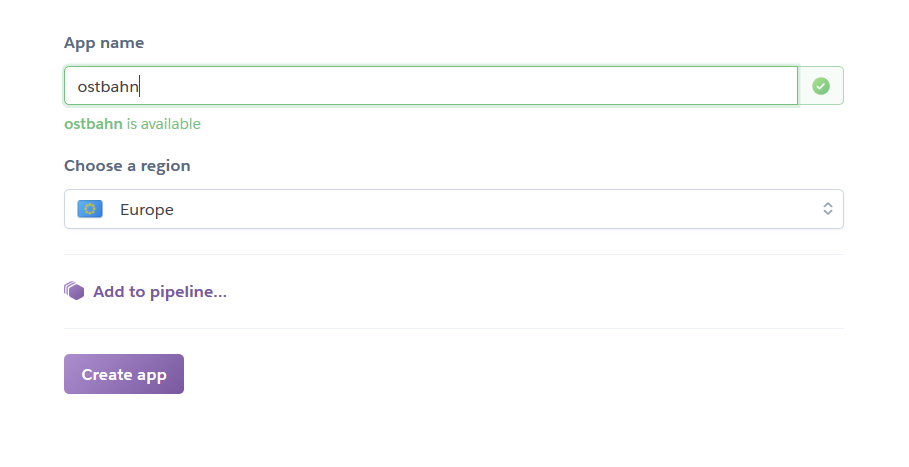
\includegraphics[width=0.7\linewidth]{images/screenshot002}
	\caption{Erstellen Dialog}
	\label{fig:screenshot002}
\end{figure}

In dem Dialog muss der Name hinzugefügt werden. Dort kann auch die Server position gewählt werden, welche auf Europa gesetz wurde.

\begin{figure}
	\centering
	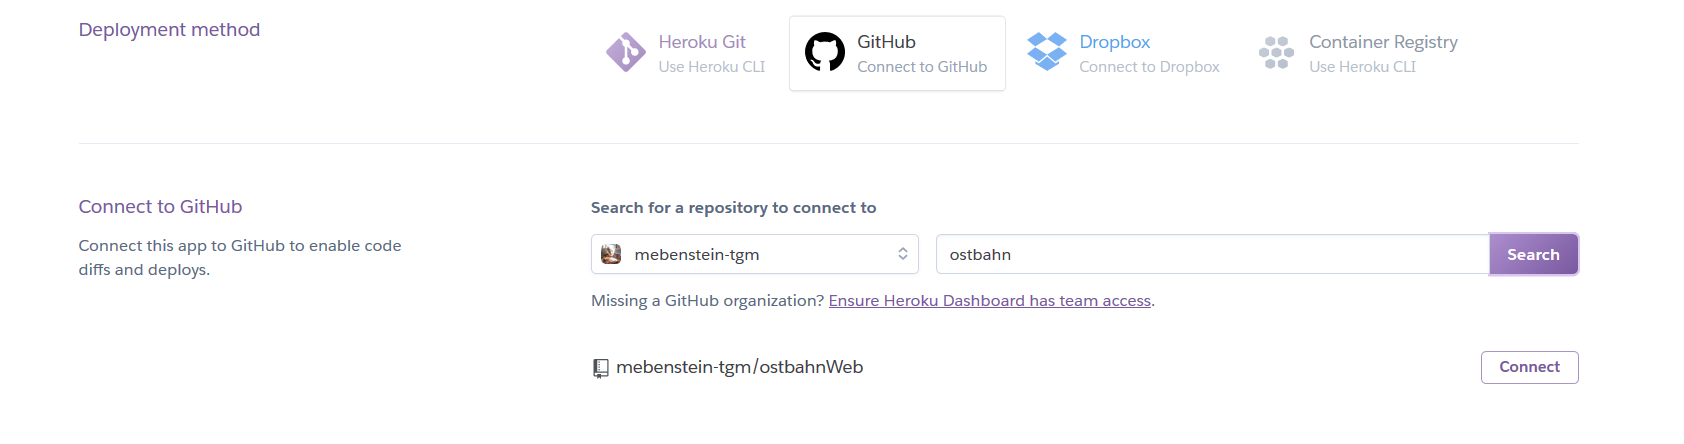
\includegraphics[width=0.7\linewidth]{images/screenshot004}
	\caption{Github connection}
	\label{fig:screenshot004}
\end{figure}

Um die Applikation zu deployen wird diese mit dem Github repository verbunden. Dafür wird das entsprechende Repository ausgewählt.\\

\begin{figure}
	\centering
	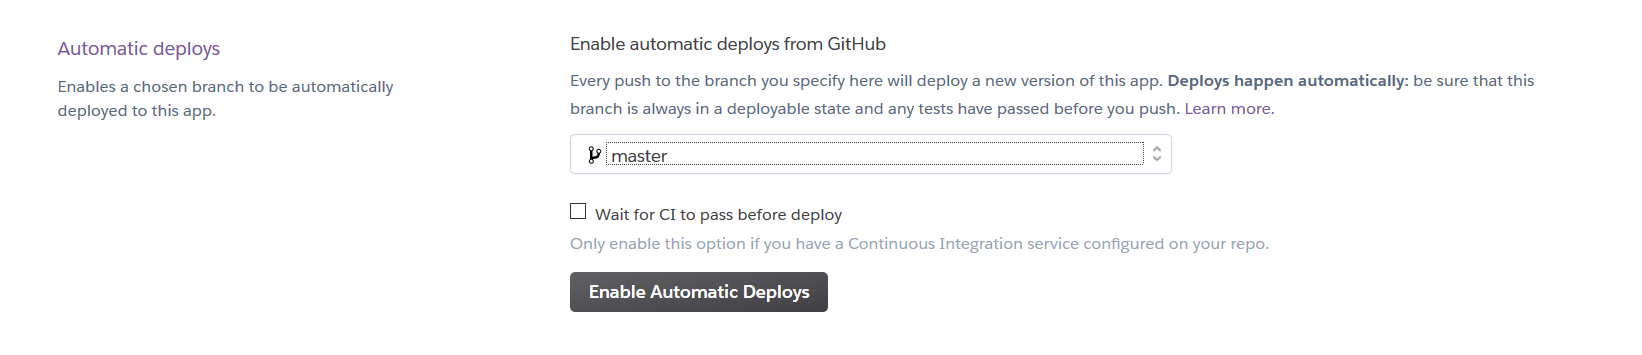
\includegraphics[width=0.7\linewidth]{images/screenshot005}
	\caption{Automatic Deployment}
	\label{fig:screenshot005}
\end{figure}

Mit dieser Konfiguration kann eingestellt werden, dass bei jedem Push die Applikation neu deployed wird.

 % Solution for the given tasks and their documentation
% \glsaddall 		% Add all glossary entries to printglossaries
\end{document}
